% -*- TeX-PDF-mode: t -*-

% Template for ICASSP-2010 paper; to be used with:
%          spconf.sty  - ICASSP/ICIP LaTeX style file, and
%          IEEEbib.bst - IEEE bibliography style file.
% --------------------------------------------------------------------------
\documentclass{article}
\usepackage{spconf,amsmath,graphicx}
\usepackage{url}
\usepackage{verbatim}
\usepackage{subfig}
%\usepackage{microtype}
\usepackage{booktabs}

% Example definitions.
% --------------------
\def\x{{\mathbf x}}
\def\L{{\cal L}}

\usepackage{color}
\newcommand{\FIXME}[2][FIXME]{\textcolor{blue}{\textbf{#1}: \emph{#2}}}

% Title.
% ------
%\title{IMPUTATION OF BEAT-ALIGNED FEATURES AND MUSIC PATTERN LEARNING}
\title{EVALUATING MUSIC SEQUENCE MODELS THROUGH MISSING DATA}
%
% Single address.
% ---------------
%\name{Thierry Bertin-Mahieux\thanks{Thanks to NSERC and some other stuff.}}
%\address{EE dept., Columbia University}
%
% For example:
% ------------
%\address{School\\
%	Department\\
%	Address}
%
% Two addresses (uncomment and modify for two-address case).
% ----------------------------------------------------------
\twoauthors {Thierry Bertin-Mahieux\sthanks{supported in part by a
    NSERC PG scholarship.}, Graham Grindlay} {Columbia University\\
  LabROSA\\ New York, USA} {Ron J. Weiss\sthanks{supported by NSF
    grant IIS-0844654 and Institute of Museum and Library Services
    grant LG-06-08-0073-08.} and Daniel P.W. Ellis} {New York
  University / Columbia University\\ MARL / LabROSA\\ New York, USA}

\begin{document}
\ninept
%
\maketitle
%
\begin{abstract}
  We investigate the task of missing data imputation in music signals
  as a means of evaluating the ability of different signal models to
  accurately capture the temporal structure of music.
  %
  We analyze beat-synchronous chroma features and compare imputation
  based on simple linear prediction to more complex
  signal models including nearest neighbor selection and
  shift-invariant probabilistic latent component analysis.
  %
  Simple predictive models perform best according to a Euclidean
  distance metric, despite producing stationary results which are not
  musically meaningful.  We therefore investigate alternate evaluation
  measures % which emphasize musical consistency
  and find that an entropy difference %information theoretic
  metric tends to correlate
  better with our %intuitive
  expectations for musically consistent reconstructions.
  %
  The imputation algorithm which performs best under this
  entropy-based metric over a large data set of popular music
  reconstructs masked sections by choosing the nearest neighbor to the
  surrounding observations within the song.
  %
  This result is consistent with the highly repetitive structure 
  found in pop music.
\end{abstract}
%
\begin{keywords}
Missing data imputation, chroma features, entropy difference,
music sequence models
\end{keywords}
%

% NSF thanks
\makeatletter{\renewcommand*{\@makefnmark}{}
\footnotetext{This work is supported by NSF grant
    IIS-0713334 and by a gift from Google, Inc.
    Any opinions, findings and conclusions or
    recommendations expressed in this material are those of the
    authors and do not necessarily reflect the views of the sponsors.}\makeatother}

\section{Introduction}
\label{sec:intro}
As with many classes of time-series data, musical signals contain
substantial amounts of complex structural information.  Given the
intricate nature of this data, learning models of music in an
unsupervised fashion is a particularly challenging task.  In addition
to musicological implications, large-scale models of music data have
numerous commercial applications, including recommendation systems,
digital rights management, and creative tools.  In many of these cases
we are interested in models that capture local patterns
(i.e. ``patches'') in the data.  Finding robust sequential patterns
may prove useful for tasks such as song similarity (recognizing songs
with similar patterns), song segmentation (labeling chorus/verse
structure), and cover song recognition (identifying songs with similar
high-level patterns).  All of these tasks would benefit from patch
models that exhibit high-level musical characteristics while remaining
faithful to the observed signal data.
%\FIXME[gg]{Do we need to back this up more?}
%Therefore, we are interested in patterns that not only explain the
%low-level signal, but also contain musical characteristics.  
However, the requirement that patches be musically sensible makes it
unclear how to evaluate the quality of this type of model.  In this
paper, we propose a task based on missing data imputation and discuss
various performance metrics which are sensitive to musically
meaningful aspects of the data.

Imputation refers to a family of techniques used to fill in missing
data entries.  Previous work on audio-related applications has
included speech denoising~\cite{Cooke1996,Raj1998}, source
separation~\cite{Reyes-Gomez2005}, bandwidth
expansion~\cite{Smaragdis2009}, and model
evaluation~\cite{Hoffman2010}.  However, much of the previous work has
focused on at most a single time-frame.
%However, to the best of
%our knowledge, previous research has only considered at most a single
%missing time frame.
%a few missing time-frequency \emph{bins}
%\FIXME[ronw]{this isn't totally fair, some of the missing
%  data speech stuff is based on imputation using HMM/CRF models. E.g. see
%  figure 3 of
%  {\footnotesize \url{http://www.ee.columbia.edu/~mjr59/AISTATS-defspec.pdf}}
%}.
The single-frame imputation problem is often somewhat easy since the
harmonic content of music tends to change more slowly than a single
frame.  However as the amount of missing data increases, the problem
becomes significantly more challenging.
%
We therefore focus on the task of \emph{multi-frame} imputation in
% many consecutive time frames
which long segments of the signal are missing.
%
Obtaining good performance on this task requires the use of a model
which can take advantage of the highly structured nature of music.  It
therefore serves as a good way to
% This allows us to
more carefully evaluate the temporal aspects of competing
models.  % needs to be reworded?
% mention real-world packet-loss case?


The difficult nature of multi-frame imputation of music data is
demonstrated in Figure \ref{fig:basic}.
Linear prediction, which
explicitly minimizes Euclidean distance, is used to impute the missing
data in Figure~\ref{fig:basic} $6$th row.  However, it is clear from
visual inspection that linear prediction yields an overly-smooth
reconstruction and is unable to predict the temporal evolution within
the missing section.
%
A more sophisticated signal model which better leverages the
surrounding context and makes use of long-term temporal information
such as knowledge of repetitions within a song (note that the missing
sequence in Figure~\ref{fig:basic} is repeated at frame 70) is
necessary to achieve a musically coherent reconstruction.
%
Unfortunately, simple algorithms such as linear prediction are often
prone to identifying poor solutions, despite optimizing standard
metrics such as Euclidean distance.
%
In this paper, we argue that a more extensive set of metrics is needed
to properly evaluate a model's ability to predict musical sequences.
%more for proper evaluation.


\section{TASK DEFINITION}
\label{sec:task}

\subsection{DATA AND FEATURES}
\label{ssec:feats}
In the experiments described below, we use a set of $5000$ songs taken
from the \emph{morecowbell.dj} dataset~\cite{Bertin-Mahieux2010a}.
This dataset contains a wide variety of (predominantly western) pop
music.  The raw audio was then converted to a chromagram
representation using the online Echo Nest
API.\footnote{\url{http://developer.echonest.com}} A chromagram is
similar in spirit to a \mbox{constant-Q} spectrogram except that pitch
content across all octaves has been folded into $12$ discrete bins,
each of which corresponds to a semitone (e.g. piano key).
%In the chroma representation, the pitch content at each point in time
%is folded into a $12$ binsintensity associated with each of the 12
%semitones (e.g. piano keys) across all octaves.
%
%One can see them as a very coarse %and noisy
%and low dimensional music transcription which captures the harmonic
%content of the signal while ignoring information related to timbre and
%instrumentation.  
%We use an online API\footnote{\url{http://developer.echonest.com}} %
%\cite{EchoNest} 
%that computes chroma from a constant-Q spectrogram.

Music naturally evolves over a time scale expressed in beats, as
opposed to the fixed-length frames commonly used in other audio
processing applications.  Beat-aligned chroma can be formed by
resampling a chromagram so that each chroma (column) vector spans a
single beat.  This representation has been successfully used for cover
song recognition~\cite{Ellis2007a}, segmentation~\cite{Weiss2010}, and
in our previous work on patch modeling~\cite{Bertin-Mahieux2010a}.  As
a post-processing step, we remove variability due to loudness by
normalizing each column to have a maximum value of one.

% ronw: this sentence is unnecessary
% Note
%that music beat tracking algorithms perform relatively well
%\cite{Davies2007} even if the task is not considered solved.

%Beat-aligned chroma features have been used for cover song recognition
%\cite{Ellis2007a} and segmentation \cite{Weiss2010}. In our previous work
%\cite{Bertin-Mahieux2010a}, we attempt to learn music patterns in that
%representation.
% Results on multi-frame imputation are done on
%In the following sections we report experimental results over 
%a random
%subset of $5000$ songs from the morecowbell.dj dataset
%\cite{Bertin-Mahieux2010a}.


%\begin{figure}[t]
%\begin{center}
%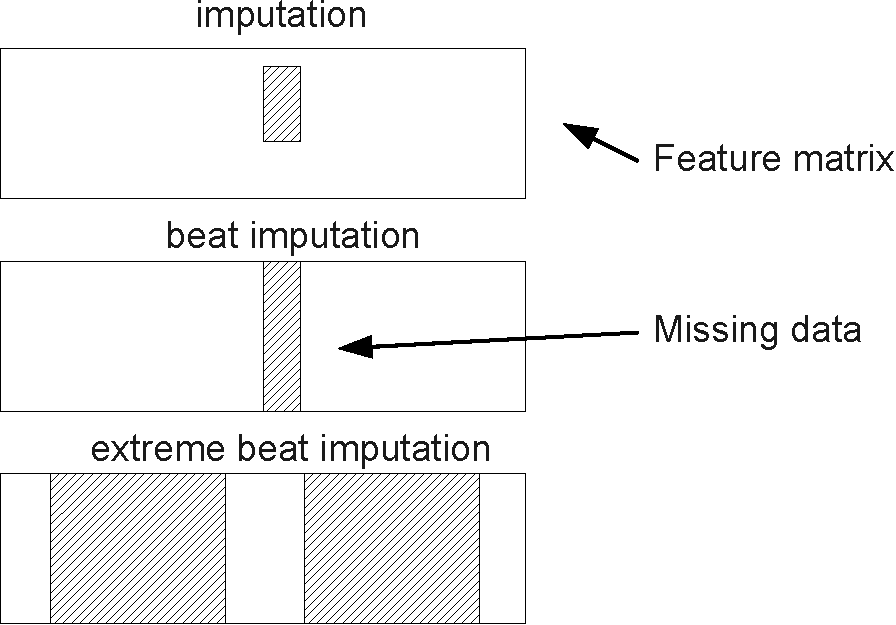
\includegraphics[width=.7\columnwidth]{type_imputation}
%\end{center}
%\caption{Imputation types.
%\label{fig:types}}
%\end{figure}

\begin{figure}[t]
\begin{center}
%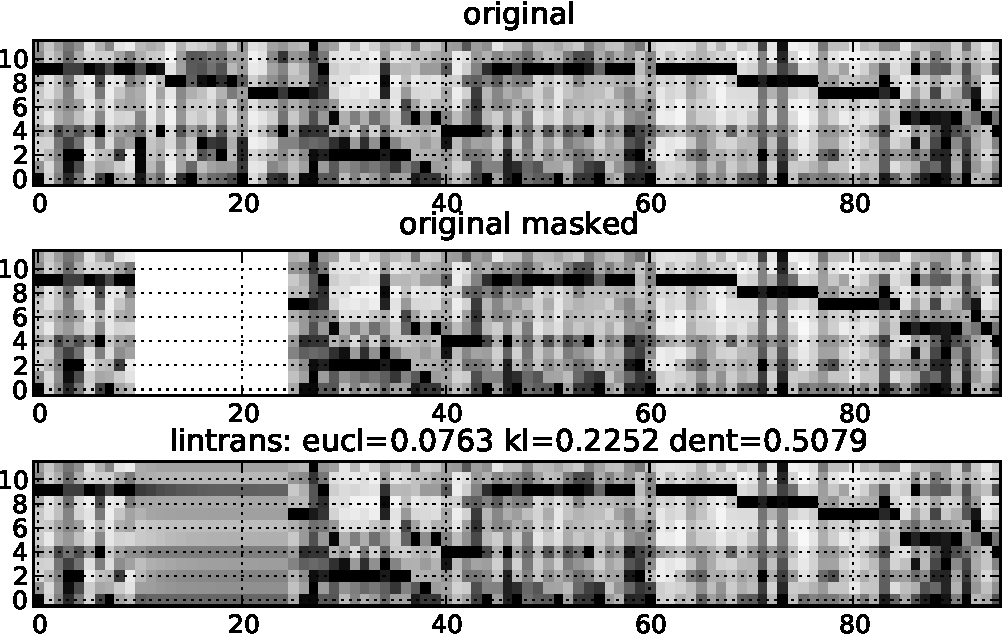
\includegraphics[width=.95\columnwidth]{basic}
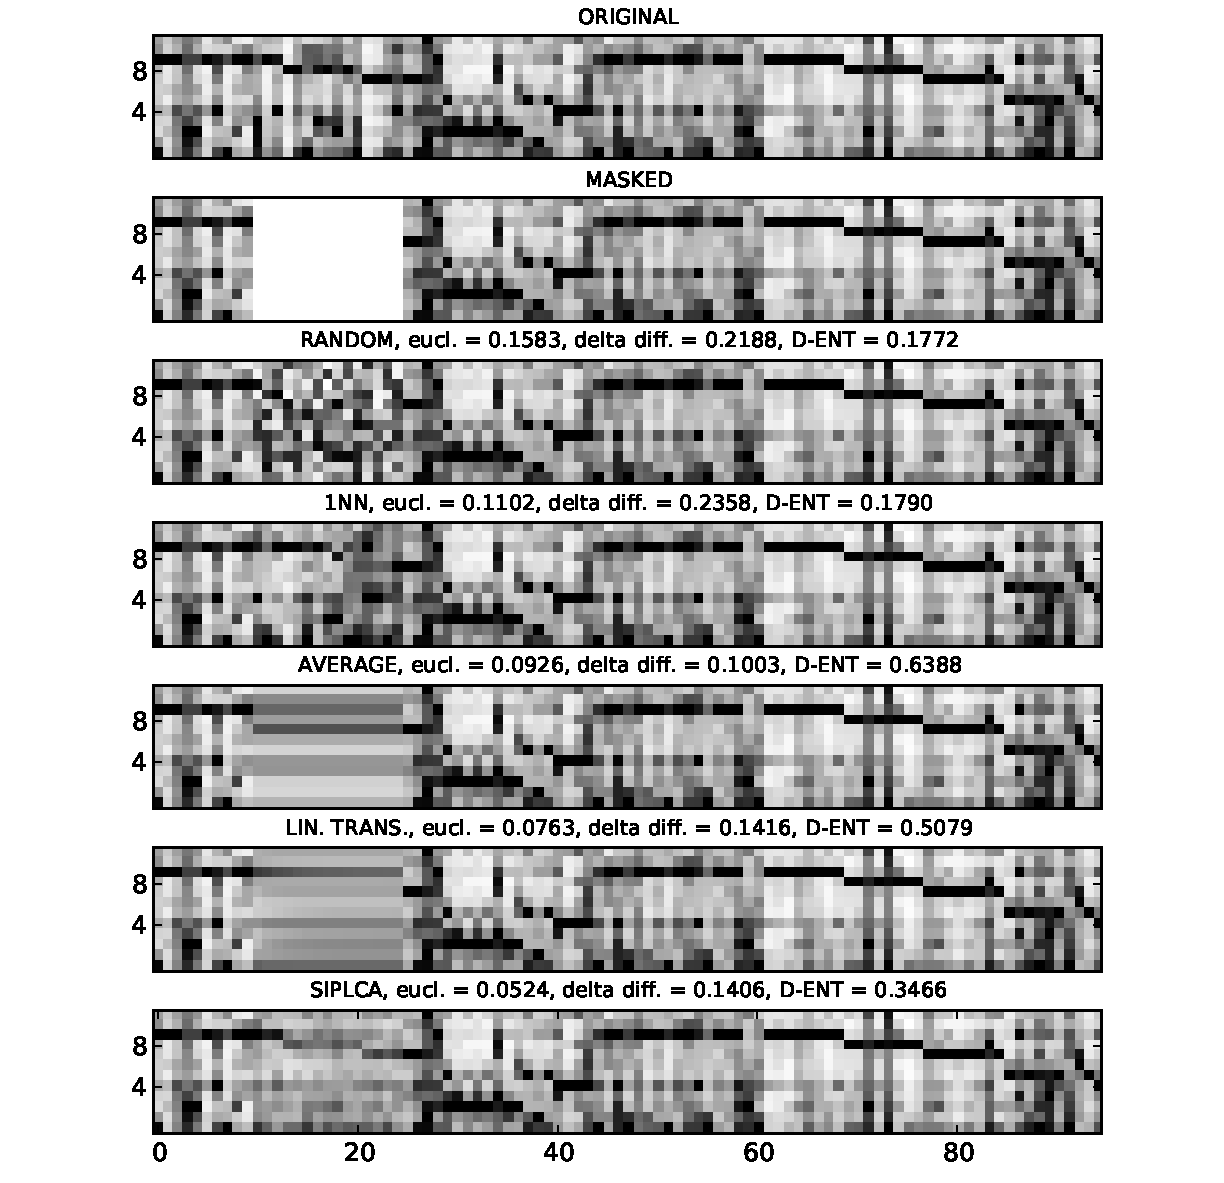
\includegraphics[width=.99\columnwidth]{basic2}
\end{center}
\caption{$15$ beats imputation example, rows are 1) original 2) original masked,
then reconstruction using 3) random 4) nearest neighbor 5) average of nearby beats
6) linear transform of one previous beat 7) SIPLCA (see Subsection \ref{ssec:algo}
for algorithmic details). Song longer than shown here.
\label{fig:basic}}
\end{figure}

% IPYTHON COMMAND TO RECREATE ABOVE FIGURE
%btchroma2 = sio.loadmat('/home/thierry/Columbia/covers80/coversongs/covers32kENmats/john_lennon+Double_Fantasy+05-I_m_Losing_You.mp3.mat')['btchroma']
%p1=185;p2=p1+15;mask=np.ones(btchroma2.shape);mask[:,p1:p2]=0.
%evaluation.plot_oneexample(btchroma2,mask,p1,p2,methods=['lintrans'],methods_args=[{'win':1}],measures=('eucl','kl','dent'),plotrange=(p1-10,p2+70))



\subsection{ALGORITHMS}
\label{ssec:algo}
As multi-beat imputation has not been studied before, we report
results on a variety of benchmark algorithms. We realize that such
methods have a low probability of success at solving the task, but
their relative performance is of interest.  Simple methods include
random where each chroma bin is drawn from a uniform $[0,1)$
distribution (Figure \ref{fig:basic}, $3$rd row).  One can also pick a
beat at random from the song, or take the average of all visible
beats. Taking the average of the beats within a certain range
of the missing patch (Figure \ref{fig:basic}, $5$th row) create a
smooth reconstruction, but still solves the case of sustained notes.

Our first trained model is linear prediction (also called linear
transform in the text) where we use $N$ previous beats to predict the
next one.  As it explicitly learns to minimize Euclidean distance on
the visible data, this methods performs very well under certain
metrics (See Figure \ref{fig:basic}). From our experiments, $N=1$ or
$N=2$ work best.

Nearest neighbor ($1$NN) is an appropriate technique
to take advantage of the repetitions within a song. By looking at the
nearby beats of the missing data, we can impute a reconstruction by
spotting a similar neighborhood. Note that instead of using the
visible part of the song, one can use a codebook made of
other songs.  $k$NN with $k>1$ is ongoing research.

Previous methods rely on local, low-level information which should not
be enough to solve multi-frame imputation. HMM or NMF should better
leverage long term dependencies and nearby information.  We experiment
with shift invariant probabilistic latent component analysis (SIPLCA)
\cite{Smaragdis2009,Weiss2010}, a probabilistic variant of convolutive
NMF. SIPLCA learn how to encode the signal as a set of overlapping
patches. 
%As a gross simplification, one
%could compare SIPLCA to a smart nearest-neighbors. However, by
%controlling the activations, i.e. the matrix deciding when and where
%to use each patch, we can hope to impute the missing data with patches
%smaller than the missing gap. This is important when the amount of
%missing data is increased as learning longer patterns is exponentially
%difficult.  
%\FIXME[ronw]{Why do the SIPLCA ``patches'' need to be
%  shorter than the amount of missing data?}  
%In our case, we use a
%hierarchical SIPLCA model which will be described in detail in a
%future publication.  
The SIPLCA algorithm extracts template chroma
patches that are consistently repeated throughout a song.  Missing
data is imputed by identifying templates consistent with the features
neighboring the missing segment.  In the case of missing segments
longer than the identified templates, our imputation algorithm
utilizes a hierarchical reconstruction scheme, whose detailed
explanation is beyond the scope of this paper.  SIPLCA for imputation
is ongoing research, we refer the interested reader to our code until
then.


%\subsection{MEASURES}
\subsection{EVALUATION METRICS}
\label{ssec:measures}
Euclidean distance is a natural first choice for evaluating
reconstruction and encoding tasks. However, as can be seen in Figure
\ref{fig:basic}, algorithms which minimize this metric do not
necessarily capture all of the relevant data statistics.  In
particular, the solution is overly smooth and longer-term temporal
patterns are poorly reconstructed.

Clearly, the simplicity of the model is largely responsible for these
issues.  However, inherent in the Euclidean distance criterion is a
preference for smooth solutions.
%There is no doubt that this poor reconstruction is in part due to
%the simplicity of the model. That said, we argue that minimizing
%Euclidean distance also leads to such reconstructions, i.e. when 
%a model is unsure of a value, it gets the most reward from a smooth
%solution.
To see why, consider the toy example of Figure \ref{fig:square}. We
impute the original one-dimensional signal, a square wave (solid
line), by two signals: a translated identical square wave (dot-dashed
line), and a constant signal (dashed line). The first signal has an
average reconstruction error of $0.50$ using Euclidean distance. The
second signal has an average error of only $0.25$, despite the fact
that it does not appear to reflect the overall shape of the original
data.

%Applied to a multidimensional signal, it implies that Euclidean
%distance rewards overly-smoothed reconstruction, thus it can be
%misleading.

The class of Minkowski distances are given by the form $d_p =
|x_1-x_2|^p$, of which the Euclidean is a special case ($p=2$).  In
general, as $p \rightarrow 0$ the resulting distance measures penalize
small values more heavily.  This has the effect of favoring
``sharper'' data sequences and is illustrated in Figure
\ref{fig:measures}.  The greyed rectangle represents the case where a
reconstruction is considered valid (error equals $0$ if it is between
some $\delta$ of the original and wrong otherwise (error equals $1$).
The Minkowski distance approximates this case when both
$\delta \rightarrow 0$ and $p \rightarrow 0$.  In the experiments described
below, we consider $p=0.5$ and $p=2$.  With $p=0.5$, on the example of
Figure \ref{fig:square}, the translated square wave is now favored
(with a reconstruction error of $0.5$) to the second signal whose
reconstruction error is now $0.71$.
%\FIXME[ronw]{elaborate on this, it's kind of unclear}

Looking at the differences between the original data and the imputed
values, it appears that we need to encourage sparsity in our
solutions.  Entropy is a natural measure of the sparsity of a
distribution and therefore it makes sense to consider related metrics.
We examined the (symmetric) Kullback-Leibler divergence, (approximate)
conditional entropy~\cite{Peng2005}, Jensen
difference~\cite{Michel1994}, and the normalize difference entropy
(D-ENT) \cite{Mentzelopoulos2004}.  The Jensen difference of two
distribution $x_1$ and $x_2$ is given by
%
$$
J(x_1,x_2) = H\left(\frac{x_1+x_2}{2}\right) - \frac{H(x_1) + H(x_2)}{2}
$$
%
where $H(x)$ denotes the entropy of $x$.  For D-ENT, we build a
$10$-bin histogram of the feature values, and compute the difference
of entropy for each bin between the original distribution and its
approximation:
$$
\mbox{D-ENT}(\mathbf{b}_1,\mathbf{b}_2) = \frac{1}{10}\sum_{i=1}^{10} \frac{\log_2 b_{1,i} - \log_2 b_{2,i}}{\log_2 b_{1,i}} % / (\mbox{\# bins})
$$
\FIXME[gg]{Use N instead of 10?}
where $\mathbf{b}_1$ is the set of bins for $x_1$.  Note that D-ENT is
not symmetric. In our experiments, we set the first vector to be the
original features. Also, the position of the different values does not
matter.

Another idea to measure the ``sharpness'' of a reconstruction compared
to the original using the first-order difference of the feature
vectors across time. We compute the  delta difference by summing
the absolute value of the delta, then taking the absolutec
difference. Once again, the position of the delta values does not
matter.

We explained above why Euclidean distance can justify disappointing
reconstructions. At the same time, we do not argue that we should
ignore or replace it. Euclidean distance measures reconstruction in a
fundamental way. We believe we need a combination of measures to
quantify the quality of music patterns, Euclidean distance being one
of them. In the next section, we investigate which measures behave in
a similar way, thus helping us to decide which ones are useful.

\begin{comment} % merged with figure 1 ``basic''
\begin{figure}[t]
\begin{center}
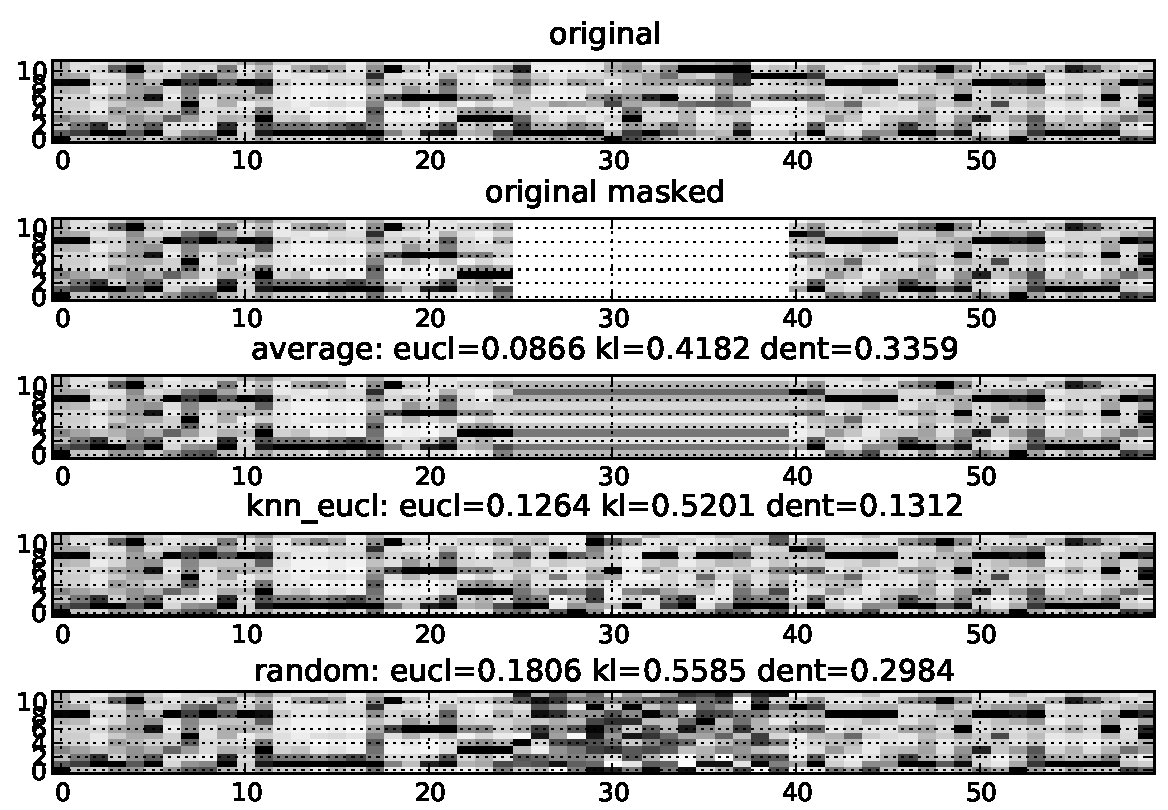
\includegraphics[width=.95\columnwidth]{avg_nn_rand}
\end{center}
\caption{Same beat imputation example as Figure \ref{fig:basic}, 
rows are 1) original 2) original masked
3) reconstruction using the average of nearby beats 4) using
nearest neighbor 5) using random.
\label{fig:avgnnrand}}
\end{figure}
\end{comment}


\begin{figure}%
\centering
\subfloat[]{%
\label{fig:measures}%
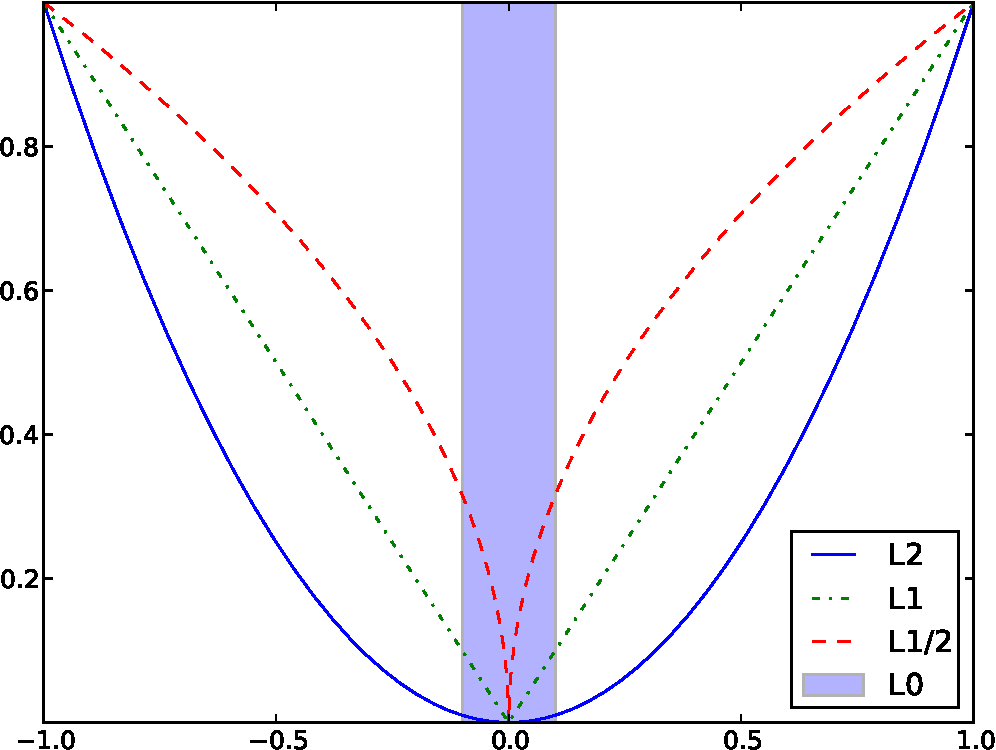
\includegraphics[width=0.485\columnwidth]{measures}} 
\hspace{0.1cm}
\subfloat[]{%
\label{fig:square}%
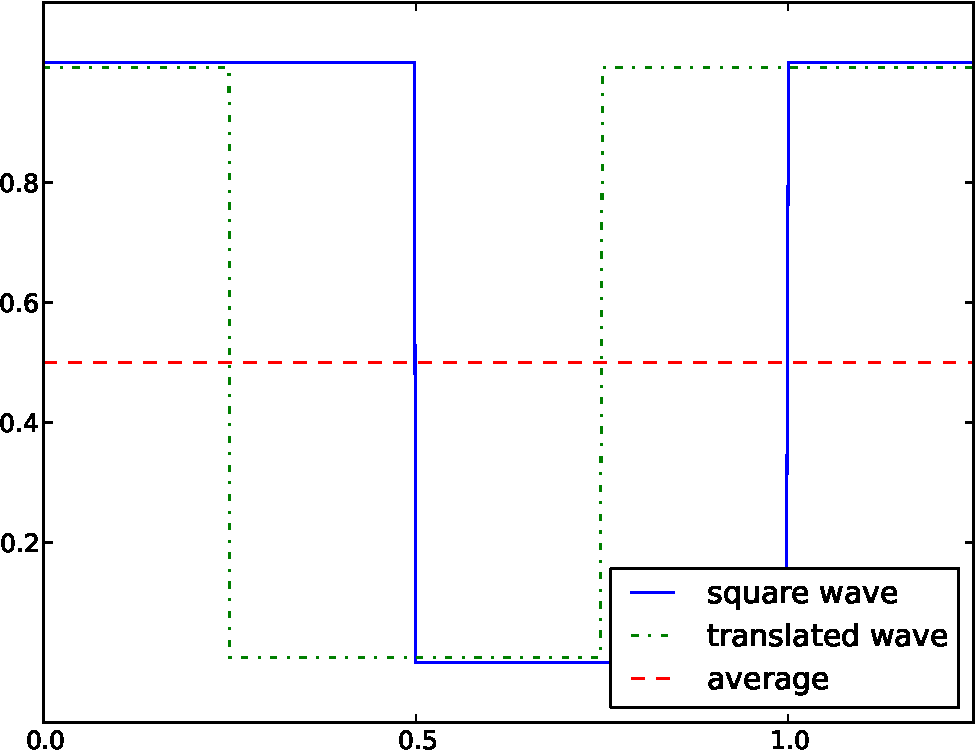
\includegraphics[width=0.475\columnwidth]{square}}%
\hspace{8pt}%
\caption{(a) Effect of different measures on one-dimensional data. (b)
  Reconstruction error between a square wave and two approximations, a
  square wave translated by a quarter of the period, and the average
  function. Average error between original and translated wave is
  always $0.5$ for any Minkowski measure $d_p$ on $[0,1]$.  For the
  average function, the errors are $0.25$, $0.5$ and $0.71$ for $d_2$,
  $d_1$ and $d_{1/2}$ respectively.}%
\label{fig:two_measures}
\end{figure}


\section{EXPERIMENTS}
\label{sec:exp}
%We present results using different algorithms for imputing masked
%sections of beat-aligned chromagrams.  The evaluation dataset is made
%of $5000$ songs from the \emph{morecowbell.dj} data described in
%\cite{Bertin-Mahieux2010a}.  We ensure that songs have a length of at
%least $100$ beats.  The masked part is chosen at random, excluding the
%first and last $30$ beats.
As we mentioned in Subsection \ref{ssec:measures}, there exist
numerous metrics to evaluate the reconstruction of a signal. Euclidean
distance is a natural first choice, but does not necessarily reward
highly-structured imputations. In order to rationalize the set of
measures we report in our experiments, we first compute the empirical
agreement of these metrics.  Pearson's correlation is defined as
$$
\rho_{X,Y}={\mathrm{cov}(X,Y) \over \sigma_X
    \sigma_Y} ={E[(X-\mu_X)(Y-\mu_Y)] \over \sigma_X\sigma_Y}
$$
$\rho_{X,Y}$. Note that $-1 \leq \rho_{X,Y} \leq 1$, and absolute
value close to $1$ means high correlation. $\rho_{X,Y}$ is computed
for many error measures based on results obtained by three methods on
two multi-frame imputation tasks. The results are shown in
Table~\ref{tab:corrs}.

The first conclusion is that a large set of measures are strongly
correlated with Euclidean distance. This includes measures not
reported here for lack space, such as KL or conditional entropy.
It might not be a surprise for
cosine distance and $d_{1/2}$ as they are similar in their
formulation. However, the fact that entropy-based measures such as KL
divergence have high correlation with Euclidean distance means it
might not serve our purpose. Two measures still stand out from the
pack.  Delta difference and D-ENT are global statistics, the first
looking at the variance in time and the second at the histogram of
values. From Table~\ref{tab:corrs}, they do seem to bring an added
value to our set of metrics.

% MEASURES IN ORDER: (bad matfile saving)
%array(['condent', 'binary', 'cos', 'eucl', 'lhalf', 'lhalf_delta', 'dent',
%       'thresh', 'thresh_delta', 'cos_delta', 'jdiff', 'kl', 'ddiff',
%       'eucl_delta', 'leven'], 
%      dtype='|S12')
\begin{table}[t]
%  \begin{small}
    \begin{center}
      \begin{tabular}{@{}l c c c c c @{}}
        \toprule
                            & Euclidean       & $d_{1/2}$ & Jensen & Delta diff. & D-ENT \\ 
        \midrule
        Euclidean           & $1$             &  &  &  &  \\ 
        $d_{1/2}$             & $0.90$          & $1$    &  &  &  \\ 
        Jensen              & $0.84$          & $0.71$ & $1$    &  &  \\ 
        %\midrule
        Delta diff. & $\mathbf{0.45}$ & $0.52$ & $0.38$ & $1$ &  \\ 
        D-ENT               & $\mathbf{0.12}$ & $0.27$ & $0.20$  & $0.52$ & $1$ \\
        %\midrule
        %Cosine      & $0.88$ & $0.76$ & $0.97$ & $-0.03$ & $0.20$ \\
        %KL          & $0.77$ & $0.64$ & $0.95$ & $-0.04$ & $0.17$ \\ 
        %Cond. Ent.  & $0.58$ & $0.68$ & $0.37$ & $0.32$  & $0.18$ \\
        %Threshold   & $0.68$ & $0.91$ & $0.51$ & $0.20$  & $0.35$ \\ 
        \bottomrule
      \end{tabular}
      \caption{Pearson correlation between measures computed using the full dataset 
               with several imputation schemes and amounts of missing data.
               Correlation is symmetric.}
      \label{tab:corrs}
    \end{center}
%  \end{small}
\end{table}

We take a closer look at the divergence between two measures in
Figure~\ref{fig:2dscore}.  It shows the performance of three methods
for different numbers of missing beats. We report Euclidean distance
and D-ENT. As we saw, they have a low empirical correlation of
$0.12$. Nearest neighbor (NN) method creates a reconstruction with a
granularity similar to the original for all mask sizes. We can assume
that D-ENT is approximately constant throughout a song. Thus, an
imputation from NN easily preserve this characteristic.  Regarding the
linear transform, it learns to minimize the Euclidean distance and
does it successfully. But as it can be seen with D-ENT and in Figure
\ref{fig:basic} $6$th row, it is done by a large amount of
smoothing. The average reconstruction has the same D-ENT as the linear
transform, which is consistent with
Figure~\ref{fig:basic}.  However, due to less
smoothing (or a less intelligent one), it does not do as well with the
Euclidean distance.

% to create this figure:
%time evaluation.plot_2_measures_dataset(test,methods=['knn_eucl','average','lintrans'],measures=['eucl','dent'],methods_args=[{'win':8},{'win':1},{'win':1}],ncols=[1,2,5,10])
\begin{figure}[t]
\begin{center}
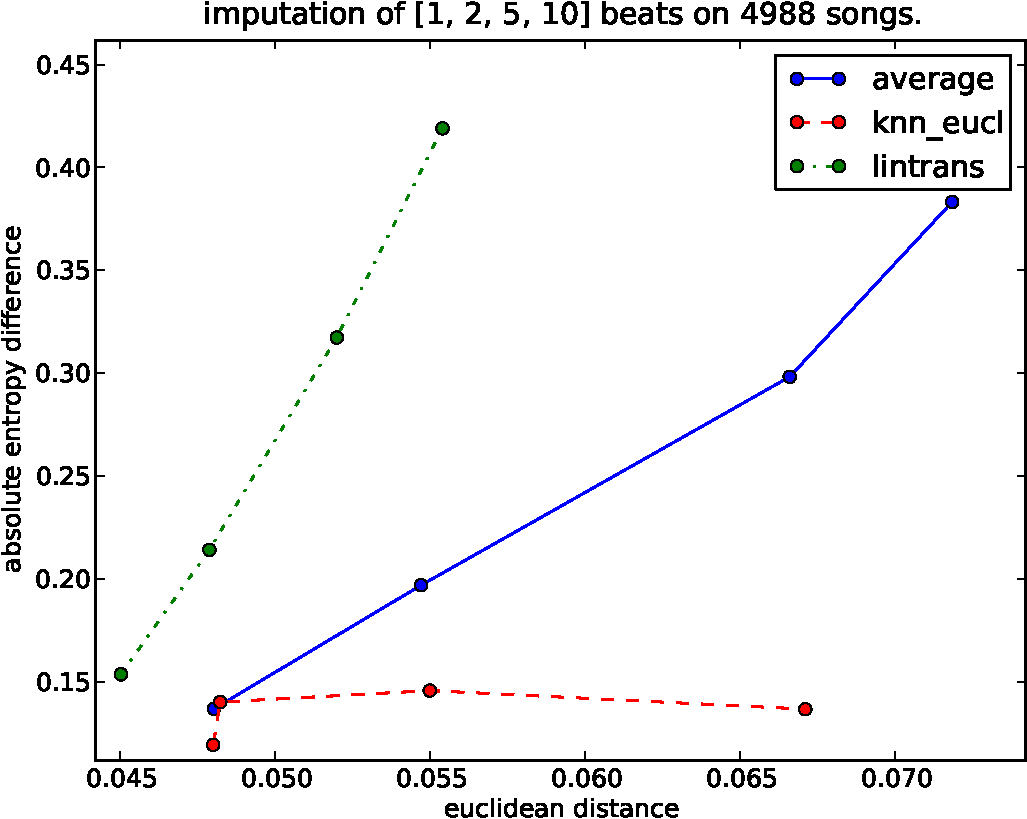
\includegraphics[width=.8\columnwidth]{recon_score_in_2d_5k}
\end{center}
\caption{Reconstruction error for $3$ methods and different
number of masked beats. Errors are D-ENT and Euclidean
distance. In all cases, the larger the number of masked beats,
the higher the Euclidean distance. Lower left is better.
\label{fig:2dscore}}
\end{figure}

Figure~\ref{fig:basic3} shows another example of imputation by
different algorithms. Algorithms are ordered according to Euclidean
distance.  However, we can see that for that case, delta difference
would have ranked first NN followed by SIPLCA whose reconstructions
seem more faithful to the original.

We now report results of a $15$ beat imputation on $5000$ songs in
Table \ref{tab:res}. The linear transform is a clear winner based on
Euclidean distance. As before, nearest neighbor's strength is to
preserve the texture of the original patch as can be seen from his
D-ENT score. We can not present all results (other number of missing
beats, other error measures, etc) due to space constraints, but they
are no serious surprises with other measures as can be expected from
Table \ref{tab:corrs}.

\begin{table}[t]
\begin{small}
\begin{center}
\begin{tabular}{|l||c|c|c|} \hline
method & Euclidean & delta diff. & D-ENT \\ \hline
random & $0.168$ & $0.135$ & $0.252$ \\
average & $0.079$ & $0.180$ & $0.430$ \\ \hline
1NN & $0.072$ & $\mathbf{0.028}$ & $\mathbf{0.123}$ \\
codebook & & & \\ \hline
lin. trans. & $\mathbf{0.056}$ & $0.170$ & $0.479$ \\
SIPLCA & $0.060$ &  & $0.395$ \\ \hline
\end{tabular}
\caption{Results on $15$ missing beats by different methods
on $5000$ songs and measured using Euclidean distance, delta
difference, and D-ENT.
\label{tab:res}}
\end{center}
\end{small}
\end{table}

% COMMENTING EVERYTHING BELOW, i.e. FIGURE WITH JUST ORIGINALS AND
% RECONSTRUCTIONS THAT NO ONE LIKES
\begin{comment}
In Figure \ref{fig:origrecon} we present specific examples of original
/ reconstruction pairs. Pay attention to the D-ENT values and the fact
that it prefers the second reconstruction.  It is due to a similar
repartition of grey-scale values troughout the patch. Once again,
this measure favors NN-like methods. Note also that delta difference
tends to reward overly-granular solution, as it is the only measure to
prefer the $3$rd reconstruction to the $2$nd one. Finally, the
reconstruction by SIPLCA is in our opinion an example of a
reconstruction that visually makes sense but get disappointing results.

\begin{figure}[t]
\begin{center}
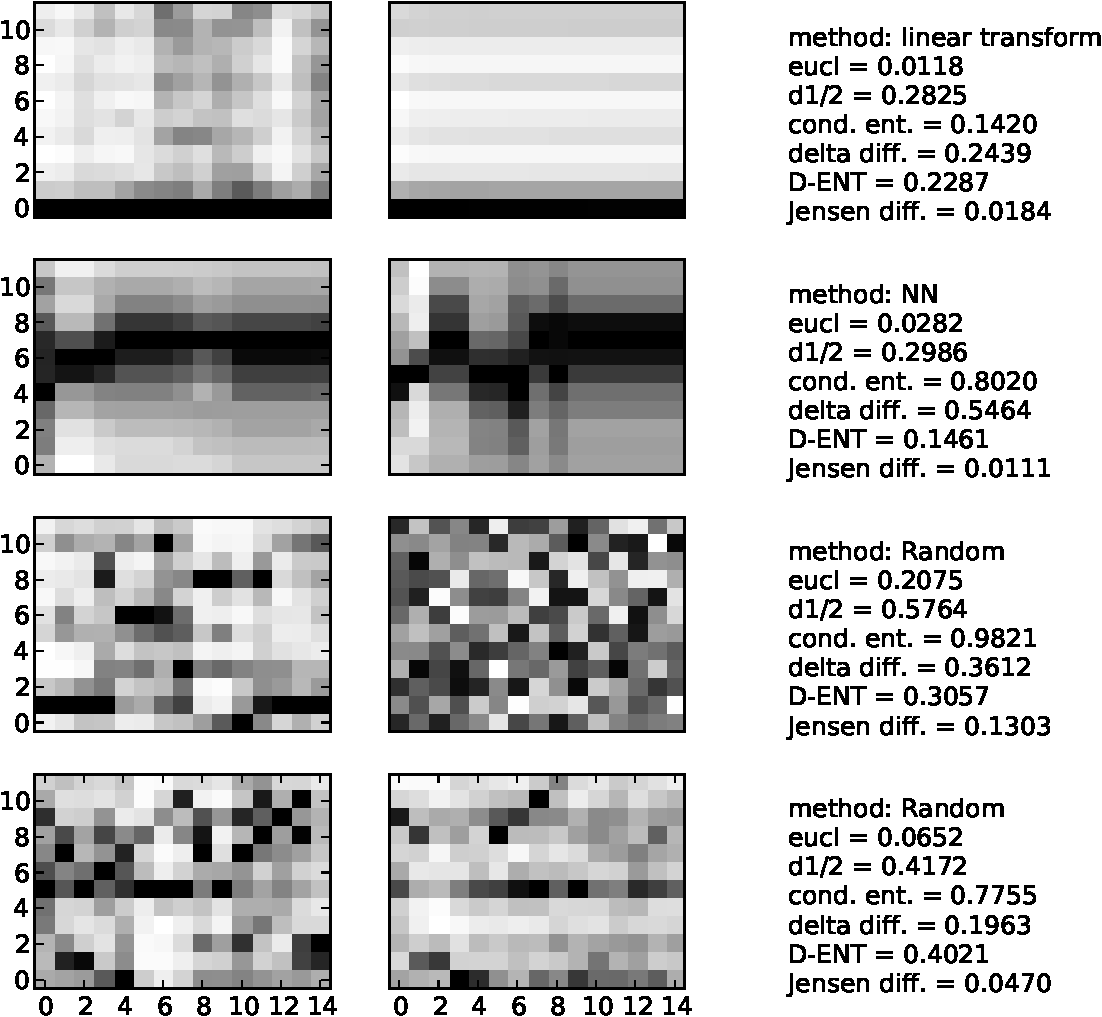
\includegraphics[width=.9\columnwidth]{original_recons}
\end{center}
\caption{Selected pairs of original patches ($1$st column)
and their reconstructions ($2$nd column). 
Method used and some error measures
reported on the right.
\label{fig:origrecon}}
\end{figure}
\end{comment}


\begin{figure}[t]
\begin{center}
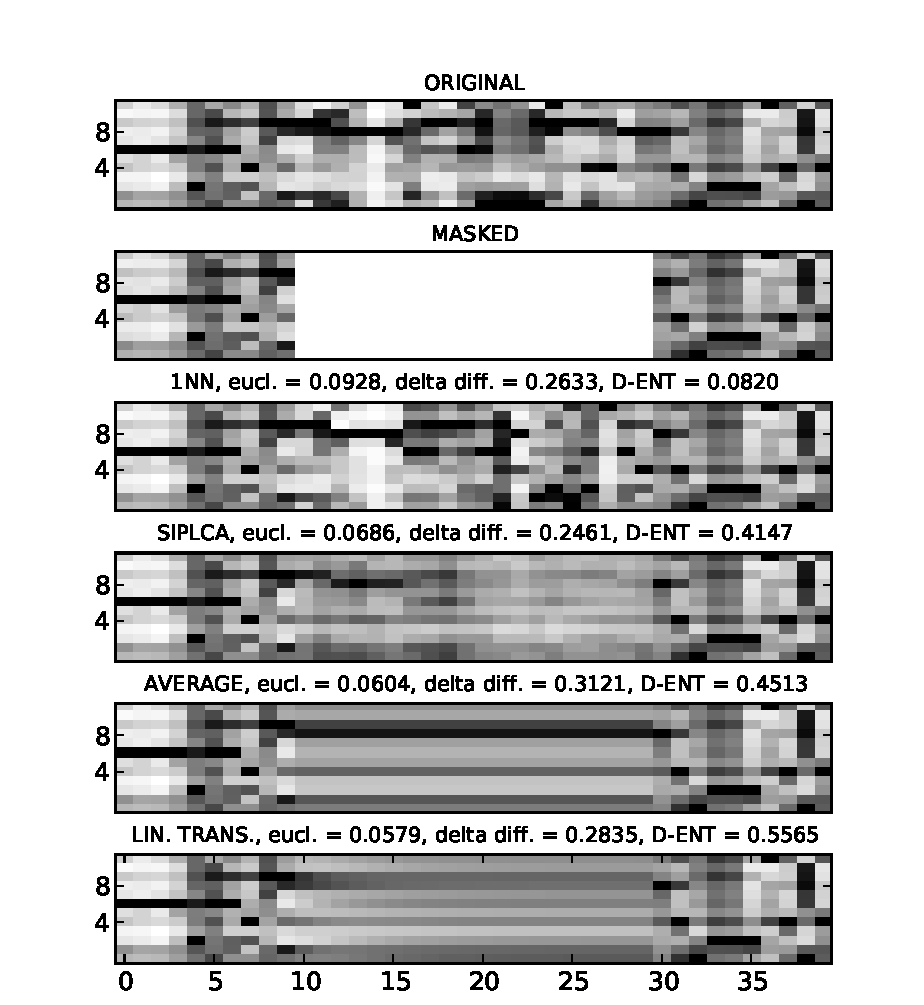
\includegraphics[width=.75\columnwidth]{basic3}
\end{center}
\caption{$20$ beats imputation example, rows are 1) original 2) original masked,
then reconstruction using same algorithms as Fig~\ref{fig:basic} (except random).
\label{fig:basic3}}
\end{figure}

\section{CONCLUSION} % AND FUTURE WORK}
\label{sec:conclusion}

We investigate the task of multi-frame imputation as a method for
evaluating models of music sequences.  
%
Key to this evaluation is the definition of appropriate performance
metrics.  
%
Experimental results over a data set of thousands of songs demonstrate
that many standard metrics for comparing feature sequences, including
Euclidean distance and Kullback-Leibler divergence, do not reliably
measure the ability of an imputation algorithm to produce musically
consistent reconstructions.  We therefore propose to complement
Euclidean distance with a measure of the entropy difference between
the original features and their reconstruction.
%
The proposed measure more consistently predicts an algorithm's ability
to produce musically coherent reconstructions that are consistent with
the original signal.
%
The best performing imputation algorithm according to Euclidean
distance often produces poor reconstructions, preferring to reuse a
single sustained chord.  The same linear prediction model performs
poorly under the proposed measures, while more sophisticated
sequence-based models show significantly better performance. 

Given an appropriate framework for evaluating music sequence models,
we intend to shift our focus to the exploration of more sophisticated
sequential imputation algorithms in the future, including hidden
Markov models and SIPLCA.
%
Our goal is to encourage researchers to further explore this task.  We
have therefore made the code and data to reproduce these results
available
online.\footnote{\scriptsize\url{http://www.columbia.edu/~tb2332/proj/imputation.html}}


%\section{ACKNOWLEDGEMENTS}
%NSERC PG grant for Thierry, something for Ron, NSF from Dan.


% References should be produced using the bibtex program from suitable
% BiBTeX files (here: strings, refs, manuals). The IEEEbib.bst bibliography
% style file from IEEE produces unsorted bibliography list.
% -------------------------------------------------------------------------
\bibliographystyle{IEEEbib}
\bibliography{tbm_bib}

\end{document}
